\documentclass{standalone}

\usepackage[OT1]{fontenc}
\renewcommand*\familydefault{\sfdefault}
\usepackage{helvet,sfmath}
\usepackage{siunitx}

\usepackage{tikz}
\usetikzlibrary{arrows,calc,patterns}
% \usetikzlibrary{intersections, calc, arrows.meta}
\usepackage{tikz,tkz-euclide}

\begin{document}
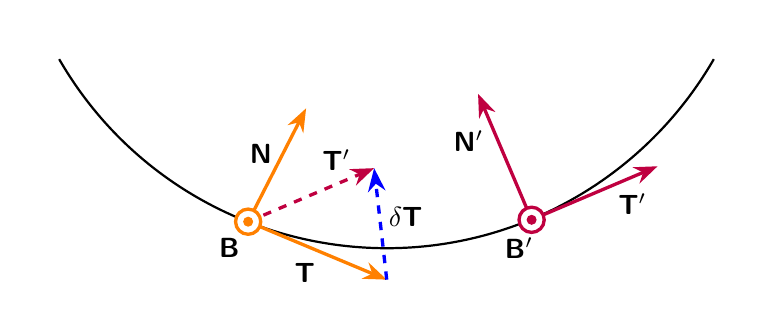
\begin{tikzpicture}[scale=0.8, >=Stealth]
    %% Background
    \draw[draw=none] (-5.5,-0.5) rectangle (5.9,3.5);

    %% Frenet Serret coordinates
    \draw[thick] (-5,3) arc (210:330:6);

    \draw[orange,very thick, ->] (-2,0.42) to (0.2,-0.5);
    \draw[orange,very thick, ->] (-2,0.42) to (-1.08,2.22);
    \draw[purple,very thick, dashed, ->] (-2,0.42) to (0,1.27);
    \draw[blue,very thick, dashed, ->] (0.2,-0.5) to (0,1.27);
    \draw[very thick,orange, fill=white] (-2,0.42) circle (0.2);
    \draw[orange, fill=orange] (-2,0.42) circle (0.07);
    
    \draw[purple,very thick, ->] (2.5,0.45) to (4.5,1.3);
    \draw[purple,very thick, ->] (2.5,0.45) to (1.65,2.45);
    \draw[very thick,purple, fill=white] (2.5,0.45) circle (0.2);
    \draw[purple, fill=purple] (2.5,0.45) circle (0.07);

    %% Notes
    \draw
    (-1.1,-0.4) node{\(\mathbf{T}\)}
    (-1.8,1.5) node{\(\mathbf{N}\)}
    (-0.6,1.4) node{\(\mathbf{T'}\)}
    (-2.3,0) node{\(\mathbf{B}\)}
    (0.5,0.5) node{\(\delta \mathbf{T}\)}
    (4.1,0.7) node{\(\mathbf{T'}\)}
    (1.5,1.7) node{\(\mathbf{N'}\)}
    (2.3,0) node{\(\mathbf{B'}\)}
    ;
\end{tikzpicture}
\end{document}
